\documentclass[border=3pt]{standalone}
% Preâmbulo compartilhado pelos diagramas TikZ da aula 9 de IHC (Princípios e Diretrizes)
\usepackage[T1]{fontenc}
\usepackage[utf8]{inputenc}
\usepackage{lmodern}
\usepackage{amsmath}
\usepackage{xcolor}
\usepackage{tikz}
\usetikzlibrary{arrows.meta,angles,quotes,decorations.pathmorphing,decorations.pathreplacing,calc,
                positioning,shapes.geometric,shapes.misc,backgrounds,fit,
                math}

% Paleta (mesma dos SVGs originais)
% Paleta da disciplina de IHC: acento roxo (#755099), da capa do livro.
% (o nome "dblue" é mantido para não alterar todos os diagramas)
\definecolor{dblue}{HTML}{755099}
\definecolor{dorange}{HTML}{B3541E}
\definecolor{dgreen}{HTML}{4A7C59}
\definecolor{dred}{HTML}{9C4B4B}
\definecolor{dcream}{HTML}{F4F1EA}
\definecolor{dshade}{HTML}{DDD7C9}

% Função gaussiana (não normalizada por padrão de escala visual)
\pgfmathdeclarefunction{gauss}{3}{%
  \pgfmathparse{1/(#3*sqrt(2*pi))*exp(-((#1-#2)^2)/(2*#3^2))}%
}

% Estilos comuns (prefixo d... para não colidir com chaves internas do pgf)
\tikzset{
  >={Stealth[length=2mm]},
  dguide/.style={gray!55, dashed, line width=0.4pt},
  daxis/.style={gray!60, line width=0.7pt, ->},
  dbody/.style={fill=black!3, draw=black!80, line width=1pt},
  dacc/.style={draw=dblue, line width=1pt},
  dlbl/.style={black!55, font=\small},
  dsub/.style={black!45, font=\footnotesize},
  dstate/.style={circle, draw=black!80, fill=dcream, line width=1pt,
                 minimum size=17mm, font=\large, inner sep=1pt},
  dobs/.style={circle, draw=black!80, fill=dshade, line width=1pt,
               minimum size=14mm, font=\large, inner sep=1pt},
  dbox/.style={rounded corners=2pt, draw=black!80, fill=dcream, line width=1pt,
               align=center, inner sep=6pt},
  dop/.style={circle, draw=black!80, fill=white, line width=1pt,
              minimum size=6mm, inner sep=0pt, font=\small},
  dtrans/.style={->, dblue, line width=1pt},
  dmeas/.style={->, dorange, line width=1pt},
  dcurve/.style={line width=1pt, dblue},
  dcurveb/.style={line width=1.4pt, dorange},
}

\begin{document}
\hyphenpenalty=10000 \exhyphenpenalty=10000 \tolerance=9999 \emergencystretch=3em
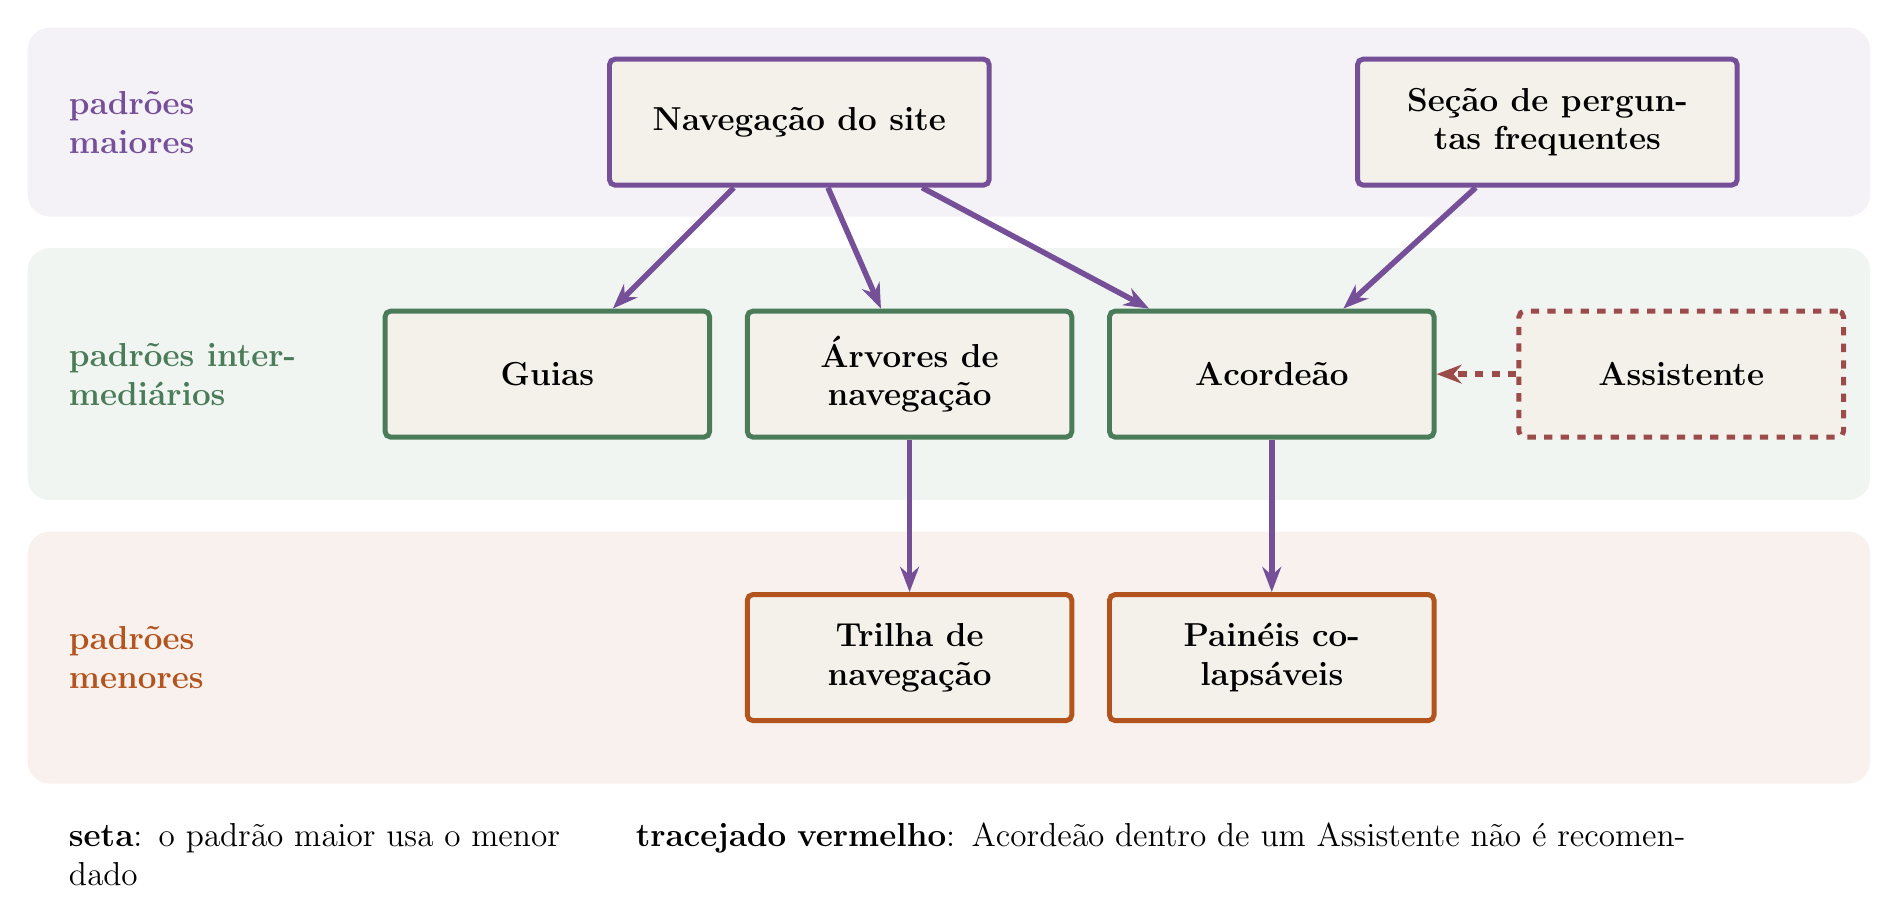
\begin{tikzpicture}[x=1cm,y=1cm]
\tikzset{n/.style={dbox, text width=3.7cm, minimum height=1.6cm, font=\large\bfseries, line width=1.8pt},
        e/.style={dtrans, line width=2pt, -{Stealth[length=3.2mm]}}}
\fill[dblue!8, rounded corners=8pt] (-0.4,7.2) rectangle (23.0,9.6);
\fill[dgreen!8, rounded corners=8pt] (-0.4,3.6) rectangle (23.0,6.8);
\fill[dorange!8, rounded corners=8pt] (-0.4,0.0) rectangle (23.0,3.2);
\node[font=\large\bfseries, dblue, anchor=west, text width=3.0cm] at (0.0,8.4) {padrões maiores};
\node[font=\large\bfseries, dgreen, anchor=west, text width=3.0cm] at (0.0,5.2) {padrões intermediários};
\node[font=\large\bfseries, dorange, anchor=west, text width=3.0cm] at (0.0,1.6) {padrões menores};
\node[n, draw=dblue, text width=4.4cm] (nav) at (9.4,8.4) {Navegação do site};
\node[n, draw=dblue, text width=4.4cm] (faq) at (18.9,8.4) {Seção de perguntas frequentes};
\node[n, draw=dgreen] (g) at (6.2,5.2) {Guias};
\node[n, draw=dgreen] (t) at (10.8,5.2) {Árvores de navegação};
\node[n, draw=dgreen] (a) at (15.4,5.2) {Acordeão};
\node[n, draw=dred, dashed] (w) at (20.6,5.2) {Assistente};
\node[n, draw=dorange] (b) at (10.8,1.6) {Trilha de navegação};
\node[n, draw=dorange] (p) at (15.4,1.6) {Painéis colapsáveis};
\draw[e] (nav) -- (g); \draw[e] (nav) -- (t); \draw[e] (nav) -- (a);
\draw[e] (faq) -- (a);
\draw[e] (t) -- (b);
\draw[e] (a) -- (p);
\draw[dred, line width=2pt, dashed, -{Stealth[length=3.2mm]}] (w.west) -- (a.east);
\node[font=\large, anchor=west, text width=21cm] at (0.0,-0.9) {\textbf{seta}: o padrão maior usa o menor \quad\quad \textbf{tracejado vermelho}: Acordeão dentro de um Assistente não é recomendado};
\end{tikzpicture}
\end{document}
